 \documentclass[a4paper,12pt]{article}
\usepackage{mathtools, amsmath, listings,graphicx, svg}
\graphicspath{ {images/} }
\begin{document}
\lstset{language=Python}

\title{A Critique on Random Graphs}

\author{Grady Ward}

\maketitle

\section*{Existing Models of Random Graphs}

The two dominant models for 'random', undirected graphs were both defined by Erdos and Reyni in TODO.
The first is a model which selects an adjacency matrix at random from the set of all square binary matrices.
The second constructs each edge with an independent and fixed probability. 
Both models have been studied at length, and they have been proven asymptotically alike. 
Though these models make intuitive sense, we ought examine why they have domainated the study of 'random' graphs.

In the random matrix model it is clear to see that properties of 'random' matrices can be applied to 'random' graphs.
Additionally, we can use some existing proofs and proof techniques in integer theory to advance 'random' graph theory by treating the matrix as a bitstring. 
This random graph generator has been useful because it links random matrix/integer theory to 'random' graph theory.

In the independently random edge model, we can easily calculate many properties of the graph that are of interest to graph theoreticians.
For example, the probability distribution of the number of triangles in a graph is a simple summation of products.
Additionally, this model succinctly describes many 'real-world' problems that do not require much imagination to dream up.
This model of random graphs has been impactful because it allows graph theoreticians to concretely discuss many of the properties that they are interested in, and connects graph theory to its applications.

In short, both models have stuck precisely because they marry an intuitive model with the tools to easily discuss the properties that their 'random' graphs have.

\subsection*{Disconnect from Algebra}

Neither model for 'random' graph generation treats graphs as algebraic objects.
It was shown by TODO in TODO that the number of matrices which represent a graph \(G\) is
\[| Matrices(G) | = \frac{N!}{| Aut(G) |}\]
where \(Aut(G)\) is the automorphism group of \(G\).
Thus, in perfectly symmetric graphs (such as \(K_i\)), there is only one way to represent \(G\).
In contrast, many other graphs only posess a trivial automorphism, and thus can be represented by \(N!\) matrices.
Thus, in the proposed 'random' generators, the odds of picking out one algebraic object can be a factor of \(N!\) larger than picking out another. 

This should make the reader question how 'random' graph generators fit into our colloquial understanding of randomness.
Common understandings of 'random selection from a set' implies uniform probability of selecting elements.
In graph theory, labeling and representation are rarely factors that impact our calculations, thus our default mode of understanding is found in most papers: 'irrespective of isomorphisms'.
Thus, we ought question the validity of these models, which heavily bias for some graphs over others by ignoring isomorphism.
The focus of this article is the quantification of the disconnects between these 'random' models, and random graphs as algebraic objects.

\subsection*{Proportion of Graphs with No Trivial Automorphisms}

The number of graphs (\(N_{Graphs}\))of a given size is still not available as a closed form, but has been computed to 19 vertices (OEIS A000088) (Column (1)).
The number of valid binary matrices that represent undirected non-looped graphs is trivially expressed as \(N_{Matrices} = 2^{.5(N^2 - N)}\) (Column (2)).
Dividing these two sequences of numbers gives us the average number of matrix representations per graph for each size of graph \(N\) (Column (3)).
Clearly, this average must fall between 1, and the maximum number of matrix representations for a single graph, which is simply \(N!\).
If we divide the average by the maximum, we see that it asymptotically is climbing to 1 (Column (4)).

This means that 'random' graph generators are closer to an algebraic concept of random as the size of the graph increases, 
as the average graph grows to asymptotically be equivalent in number of representations to the maximum.
The simplest interpretation of the data in column four is the 
For small graphs, \(N \in [2, 8]\), the fit of 'random' graph generators to graphs as objects is at its poorest.

\begin{tabular}{ r | r | r || r ||| r}
  \(N\) & (1) \(N_{Graphs}\) & (2) \(N_{Matrices}\) & (3) \(Avg(Mats(G))\) & (4) = (3) / \(N!\) \\
  \hline			
  0 & \(1\) & \(1\) & \(1.000\) & 1.00000 \\
  1 & \(1\) & \(1\) & \(1.000\) & 1.00000 \\
  2 & \(2\) & \(2\) & \(1.000\) & 0.50000 \\
  3 & \(4\) & \(8\) & \(2.000\) & 0.33333 \\
  4 & \(11\) & \(64\) & \(5.800\) & 0.24242 \\
  5 & \(34\) & \(1028\) & \(30.12\) & 0.25098 \\
  6 & \(156\) & \(3.2 * 10^4\) & \(210.0\) & 0.29174 \\
  7 & \(1044\) & \(2.1 * 10^6\) & \(2009\) & 0.39856 \\
  8 & \(1.2 * 10^{4}\) & \(2.7 * 10^{8}\) & \(2.2 * 10^{3}\) & 0.53925 \\
  9 & \(2.7 * 10^{5}\) & \(6.9 * 10^{10}\) & \(2.5 * 10^{5}\) & 0.68946 \\
  10 & \(1.2 * 10^{7}\) & \(3.5 * 10^{13}\) & \(2.9 * 10^{6}\) & 0.80764 \\
  11 & \(1.0 * 10^{9}\) & \(3.6 * 10^{16}\) & \(3.5 * 10^{7}\) & 0.88577 \\
  12 & \(1.7 * 10^{11}\) & \(7.4 * 10^{19}\) & \(4.5 * 10^{8}\) & 0.93308 \\
  13 & \(5.1 * 10^{13}\) & \(3.0 * 10^{23}\) & \(6.0 * 10^{9}\) & 0.96106 \\
  14 & \(2.9 * 10^{16}\) & \(2.5 * 10^{27}\) & \(8.5 * 10^{10}\) & 0.97749 \\
  15 & \(3.1 *10^{19}\) & \(4.0 * 10^{31}\) & \(1.3 * 10^{12}\) & 0.98708 \\
  16 & \(6.4 * 10^{22}\) & \(1.3 * 10^{36}\) & \(2.1 * 10^{13}\) & 0.99264 \\
  17 & \(2.5 * 10^{26}\) & \(8.7 * 10^{40}\) & \(3.5 * 10^{14}\) & 0.99584 \\
  18 & \(1.8 * 10^{30}\) & \(1.1 * 10^{46}\) & \(6.4 * 10^{15}\) & 0.99766 \\
  19 & \(2.5 * 10^{34}\) & \(3.0 * 10^{51}\) & \(1.2 * 10^{17}\) & 0.99869 \\
  \hline  
\end{tabular}

\begin{figure}[htbp]
  \centering
  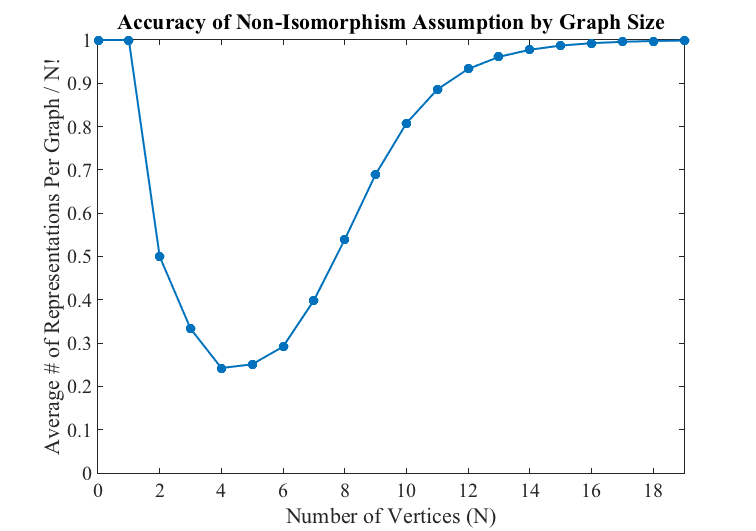
\includegraphics[scale=.45]{accuracy-of-assumption}
\end{figure}


\end{document}